\documentclass[10.5pt,a4paper]{article}

\usepackage[margin=1.9cm]{geometry}
\usepackage{fontspec}
\usepackage{titlesec}
\usepackage{enumitem}
\usepackage{xcolor}
\usepackage{hyperref}
\usepackage{tabularx}
\usepackage{graphicx}

\setmainfont{Malgun Gothic}

\definecolor{accent}{HTML}{2C5F8A}
\definecolor{textgray}{HTML}{444444}

\hypersetup{colorlinks=true, urlcolor=accent, linkcolor=accent}

\pagestyle{empty}
\setlength{\parindent}{0pt}

\titleformat{\section}
  {\large\bfseries\color{accent}}
  {}{0em}{}
  [{\color{accent!40}\titlerule[0.8pt]}]
\titlespacing*{\section}{0pt}{1.0em}{0.6em}

\newcommand{\entry}[3]{%
  \textbf{#1} \hfill \textcolor{textgray}{#2}\\
  \textcolor{textgray}{#3}\par\vspace{0.35em}
}

\newcommand{\fund}[3]{%
  \textbf{#1} \hfill \textcolor{textgray}{#2}\\
  \textcolor{textgray}{$\cdot$\ #3}\par\vspace{0.35em}
}

% Malgun Gothic has no italic shape, so publication venue lines are set
% upright rather than falling back to regular weight mid-italic.
\newcommand{\pub}[4]{%
  \textbf{#1}\\
  #2\\
  \textcolor{textgray}{#3}#4\par\vspace{0.6em}
}

\begin{document}

\noindent
\begin{minipage}[c]{0.75\textwidth}
  {\Huge\bfseries 김윤호}\par
  \vspace{0.5em}
  \color{textgray}
  rladbsgh797210@gmail.com
  \;\textbar\;
  010-2377-3059\par
  \vspace{0.2em}
  \href{https://github.com/QAZyunho}{github.com/QAZyunho}
  \;\textbar\;
  \href{https://scholar.google.com/citations?user=fFWoy8gAAAAJ&hl=en}{Google Scholar}
\end{minipage}%
\hfill
\begin{minipage}[c]{0.2\textwidth}
  \raggedleft
  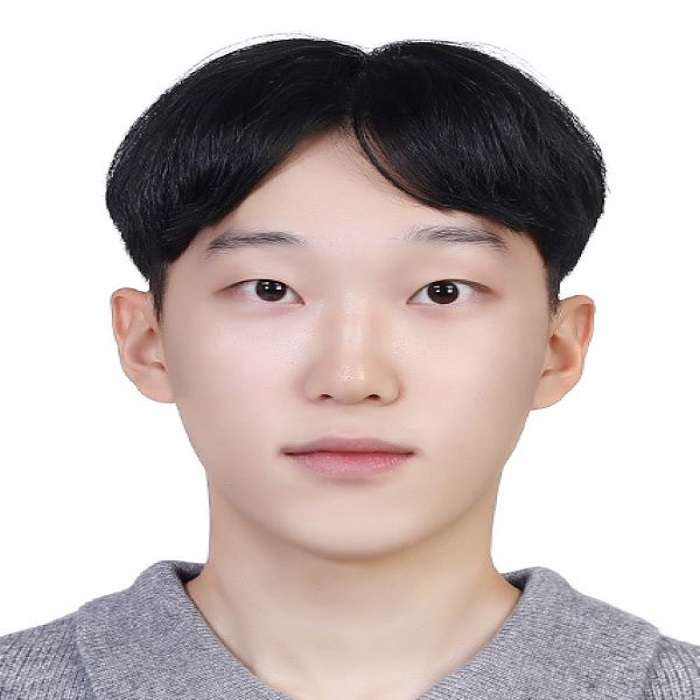
\includegraphics[width=2.6cm]{../static/images/picture.jpg}
\end{minipage}

\vspace{0.8em}

\section{학력}

\entry{Gwangju Institute of Science and Technology (GIST)}{2025.03 -- 현재}
{AI융합학과 석사과정 \,\textbar\; Data Science Lab, Sundong Kim 교수님 지도\\[0.2em]학점: 4.5/4.5}

\entry{Gwangju Institute of Science and Technology (GIST)}{2019.03 -- 2025.02}
{전기전자컴퓨터공학부 학사\\[0.2em]학점: 3.99/4.5}

\entry{University of California, Berkeley}{2023.06 -- 2023.08}
{교환학생, Summer Session\\[0.2em]학점: 3.50/4.0}

\section{펀딩 및 장학금}

\fund{National Research Foundation of Korea Funding, NRF}{2025.09 -- 2026.08}
{한국연구재단(NRF)을 통해 석사과정생으로서 연구비 ₩12,000,000 지원받음}

\fund{Korean Government Scholarships, GIST College}{2025.03 -- 현재}
{GIST 대학원생 대상 장학금}

\fund{Korean Government Scholarships, GIST College}{2019.03 -- 2025.02}
{GIST 학부생 대상 장학금}

\fund{Scholarship for Summer Session Abroad (UC Berkeley)}{2023.06 -- 2023.08}
{해외 하계 세션 참여 학생 대상 장학금}

\section{학술 활동}

\entry{GIST Global Internship Program (GIP) -- 멘토}{2025.06 -- 2025.08}
{여름 인턴 1명을 2개월간 멘토링}

\entry{GIST Summer Undergraduate Research Fellowship (G-SURF) -- 학부연구생}{2024.06 -- 2024.08}
{GIST Data Science Lab에서 Sundong Kim 교수님과 Jaehyun Park의 지도 하에 오프라인 강화학습(VAE/LDCQ)의 잠재 공간 표현 연구 수행}

\section{출판물}

\pub{On the Role of Proposal Support in Diffusion-Based Offline RL for Sequential Decision-Making}
{Yunho Kim, Jaehyun Park, Heejun Kim, Sejin Kim, Byung-Jun Lee, Sundong Kim}
{ICML 2026 Workshop DEMO}{}

\pub{Diffusion-Guided Q-Learning for Offline RL: Adaptive Revaluation for Long-Horizon Decision Making}
{Jaehyun Park, Yunho Kim, Sejin Kim, Byung-Jun Lee, Sundong Kim}
{CoRL 2025 Workshop LEAP}{}

\pub{거대언어모델의 추론능력 평가를 위한 MC-LARC 데이터셋}
{신동현, 황산하, 이석기, 김윤호, 이승필, 김선동}
{한국소프트웨어종합학술대회 (KSC 2023)}{\,\textbar\; 2023}

\section{스킬}

\textbf{언어:} 한국어 (모국어), 영어 (TOEIC Speaking IH(140) \href{https://qazyunho.github.io/website/certificates/TOEIC_Speaking_Score.pdf}{[증명서]})\par\vspace{0.4em}
\textbf{프로그래밍:} Python, C/C++

\end{document}
